\begin{appendices}

\chapter{Source Code}

\href{https://github.com/xTVaser/web-threat-thesis}{All source code and testing data sets are available online open-source under the GPLv2 license.}

\chapter{Parser Documentation} \label{app:parserDocumentation}

\chapter{Genetic Algorithm Documentation} \label{app:geneticDocumentation}

\chapter{Regular Expression Documentation} \label{app:regex}
lorem

\chapter{Full Genetic Algorithm Testing Results} \label{app:geneticFullResults}
\section{Full Text-Based Results}
\subsection{Population Size}
\begin{table}[h]
	\centering
	\begin{tabular}{|p{1.5in}|p{1in}|p{1in}|p{1in}|}
	\hline
	\textbf{Population Size} & \textbf{Successful Detection Rate (\%)} & \textbf{False Positive Rate (\%)} & \textbf{Incorrect Detection Rate (\%)}  \\
	\hhline{|=|=|=|=|}
	300 & 19.00 & 1.46 & 3.48 \\
	\hline
	600 & 28.51 & 2.33 & 3.86 \\
	\hline
	1200 & 48.77 & 44.53 & 55.57 \\
	\hline
	2500 & 75.46 & 21.80 & 32.68 \\
	\hline
	5000 & 90.95 & 6.86 & 14.30 \\
	\hline
	\end{tabular}
	\caption{Text based effects of population size on SQLi detection}
\end{table}
\begin{table}[h]
	\centering
	\begin{tabular}{|p{1.5in}|p{1in}|p{1in}|p{1in}|}
	\hline
	\textbf{Population Size} & \textbf{Successful Detection Rate (\%)} & \textbf{False Positive Rate (\%)} & \textbf{Incorrect Detection Rate (\%)}  \\
	\hhline{|=|=|=|=|}
	300 & 2.28 & 0.06 & 0.02 \\
	\hline
	600 & 23.68 & 0.06 & 0.02 \\
	\hline
	1200 & 39.04 & 0.13 & 0.03 \\
	\hline
	2500 & 55.71 & 18.53 & 25.1 \\
	\hline
	5000 & 47.51 & 0.26 & 0.08 \\
	\hline
	\end{tabular}
	\caption{Text based effects of population size on XSS detection}
\end{table}
\begin{table}[h]
	\centering
	\begin{tabular}{|p{1.5in}|p{1in}|p{1in}|p{1in}|}
	\hline
	\textbf{Population Size} & \textbf{Successful Detection Rate (\%)} & \textbf{False Positive Rate (\%)} & \textbf{Incorrect Detection Rate (\%)}  \\
	\hhline{|=|=|=|=|}
	300 & 9.69 & 0.00 & 0.00 \\
	\hline
	600 & 21.13 & 0.00 & 0.00 \\
	\hline
	1200 & 35.11 & 0 & 0.01 \\
	\hline
	2500 & 49.20 & 0 & 0.00 \\
	\hline
	5000 & 65.15 & 0 & 0.35 \\
	\hline
	\end{tabular}
	\caption{Text based effects of population size on RFI detection}
\end{table}

\newpage
\subsection{Generations}

\begin{table}[hp]
	\centering
	\begin{tabular}{|p{1.5in}|p{1in}|p{1in}|p{1in}|}
	\hline
	\textbf{Number of Generations} & \textbf{Successful Detection Rate (\%)} & \textbf{False Positive Rate (\%)} & \textbf{Incorrect Detection Rate (\%)}  \\
	\hhline{|=|=|=|=|}
	1 & 76.57 & 41.13 & 53.33 \\
	\hline
	50 & 49.00 & 3.40 & 5.67 \\
	\hline
	100 & 54.66 & 3.93 & 5.20 \\
	\hline
	500 & 47.60 & 15.00 & 12.48 \\
	\hline
	1000 & 52.06 & 3.80 & 5.21 \\
	\hline
	\end{tabular}
	\caption{Text based effects of the number of generations on SQLi detection}
\end{table}

\begin{table}[h]
	\centering
	\begin{tabular}{|p{1.5in}|p{1in}|p{1in}|p{1in}|}
	\hline
	\textbf{Number of Generations} & \textbf{Successful Detection Rate (\%)} & \textbf{False Positive Rate (\%)} & \textbf{Incorrect Detection Rate (\%)}  \\
	\hhline{|=|=|=|=|}
	1 & 72.24 & 70.06 & 83.46 \\
	\hline
	50 & 21.26 & 0.13 & 0.03 \\
	\hline
	100 & 37.08 & 0.13 & 0.01 \\
	\hline
	500 & 0.11 & 14.86 & 8.25 \\
	\hline
	1000 & 17.80 & 18.26 & 25.03 \\
	\hline
	\end{tabular}
	\caption{Text based effects of the number of generations on RFI detection}
\end{table}

\begin{table}[h]
	\centering
	\begin{tabular}{|p{1.5in}|p{1in}|p{1in}|p{1in}|}
	\hline
	\textbf{Number of Generations} & \textbf{Successful Detection Rate (\%)} & \textbf{False Positive Rate (\%)} & \textbf{Incorrect Detection Rate (\%)}  \\
	\hhline{|=|=|=|=|}
	1 & 42.24 & 0.00 & 0.01 \\
	\hline
	50 & 31.13 & 0.00 & 0.01 \\
	\hline
	100 & 39.04 & 18.40 & 32.38 \\
	\hline
	500 & 42.95 & 18.40 & 32.54 \\
	\hline
	1000 & 33.44 & 0.00 & 0.00 \\
	\hline
	\end{tabular}
	\caption{Text based effects of the number of generations on RFI detection}
\end{table}

\newpage
\subsection{Mutation Rate}

\begin{table}[h]
	\centering
	\begin{tabular}{|p{1.5in}|p{1in}|p{1in}|p{1in}|}
	\hline
	\textbf{Mutation Rate (\%)} & \textbf{Successful Detection Rate (\%)} & \textbf{False Positive Rate (\%)} & \textbf{Incorrect Detection Rate (\%)}  \\
	\hhline{|=|=|=|=|}
	0.00 & 32.53 & 32.33 & 41.36 \\
	\hline
	0.10 & 52.37 & 3.13 & 5.93 \\
	\hline
	0.25 & 60.84 & 14.73 & 15.67 \\
	\hline
	0.50 & 48.46 & 3.66 & 5.07 \\
	\hline
	1.00 & 54.46 & 3.80 & 6.12 \\
	\hline
	\end{tabular}
	\caption{Text based effects of mutation rate on SQLi detection}
\end{table}

\begin{table}[h]
	\centering
	\begin{tabular}{|p{1.5in}|p{1in}|p{1in}|p{1in}|}
	\hline
	\textbf{Mutation Rate (\%)} & \textbf{Successful Detection Rate (\%)} & \textbf{False Positive Rate (\%)} & \textbf{Incorrect Detection Rate (\%)}  \\
	\hhline{|=|=|=|=|}
	0.00 & 25.64 & 15.06 & 8.31 \\
	\hline
	0.10 & 64.31 & 0.33 & 0.06 \\
	\hline
	0.25 & 51.02 & 15.06 & 8.32 \\
	\hline
	0.50 & 24.17 & 0.00 & 0.01 \\
	\hline
	1.00 & 5.75 & 0.13 & 0.03 \\
	\hline
	\end{tabular}
	\caption{Text based effects of mutation rate on XSS detection}
\end{table}

\begin{table}[h]
	\centering
	\begin{tabular}{|p{1.5in}|p{1in}|p{1in}|p{1in}|}
	\hline
	\textbf{Mutation Rate (\%)} & \textbf{Successful Detection Rate (\%)} & \textbf{False Positive Rate (\%)} & \textbf{Incorrect Detection Rate (\%)}  \\
	\hhline{|=|=|=|=|}
	0.00 & 23.66 & 0.00 & 0.04 \\
	\hline
	0.10 & 35.75 & 0.00 & 0.02 \\
	\hline
	0.25 & 32.37 & 0.00 & 0.02 \\
	\hline
	0.50 & 32.28 & 0.00 & 0.15 \\
	\hline
	1.00 & 32.71 & 0.00 & 0.45 \\
	\hline
	\end{tabular}
	\caption{Text based effects of mutation rate on RFI detection}
\end{table}

\newpage
\subsection{Elitist Pool}

\begin{table}[h]
	\centering
	\begin{tabular}{|p{1.5in}|p{1in}|p{1in}|p{1in}|}
	\hline
	\textbf{Elitist Pool Size (\%)} & \textbf{Successful Detection Rate (\%)} & \textbf{False Positive Rate (\%)} & \textbf{Incorrect Detection Rate (\%)}  \\
	\hhline{|=|=|=|=|}
	0 & 8.40 & 0.73 & 0.14 \\
	\hline
	2 & 20.33 & 1.26 & 6.54 \\
	\hline
	5 & 61.31 & 6.40 & 12.62 \\
	\hline
	10 & 83.53 & 22.33 & 33.14 \\
	\hline
	25 & 91.37 & 9.06 & 14.52 \\
	\hline
	\end{tabular}
	\caption{Text based effects of the size of elitist pool on SQLi detection}
\end{table}

\begin{table}[h]
	\centering
	\begin{tabular}{|p{1.5in}|p{1in}|p{1in}|p{1in}|}
	\hline
	\textbf{Elitist Pool Size (\%)} & \textbf{Successful Detection Rate (\%)} & \textbf{False Positive Rate (\%)} & \textbf{Incorrect Detection Rate (\%)}  \\
	\hhline{|=|=|=|=|}
	0 & 2.68 & 14.93 & 8.27 \\
	\hline
	2 & 0.57 & 0.06 & 0.01 \\
	\hline
	5 & 28.48 & 14.933 & 8.25 \\
	\hline
	10 & 70.22 & 0.26 & 0.03 \\
	\hline
	25 & 87.08 & 18.53 & 25.07 \\
	\hline
	\end{tabular}
	\caption{Text based effects of the size of elitist pool on XSS detection}
\end{table}

\begin{table}[h]
	\centering
	\begin{tabular}{|p{1.5in}|p{1in}|p{1in}|p{1in}|}
	\hline
	\textbf{Elitist Pool Size (\%)} & \textbf{Successful Detection Rate (\%)} & \textbf{False Positive Rate (\%)} & \textbf{Incorrect Detection Rate (\%)}  \\
	\hhline{|=|=|=|=|}
	0 & 1.28 & 0.00 & 0.00 \\
	\hline
	2 & 11.53 & 0.00 & 0.01 \\
	\hline
	5 & 35.46 & 18.40 & 0.03 \\
	\hline
	10 & 56.91 & 18.40 & 0.00 \\
	\hline
	25 & 72.35 & 0.00 & 0.00 \\
	\hline
	\end{tabular}
	\caption{Text based effects of the size of elitist pool on RFI detection}
\end{table}

\newpage
\subsection{Combining Multiple Signature Sets}

\begin{table}[h]
	\centering
	\begin{tabular}{|p{1.5in}|p{1in}|p{1in}|p{1in}|}
	\hline
	\textbf{Number of Iterations} & \textbf{Successful Detection Rate (\%)} & \textbf{False Positive Rate (\%)} & \textbf{Incorrect Detection Rate (\%)}  \\
	\hhline{|=|=|=|=|}
	1 & 97.40 & 20.40 & 33.68 \\
	\hline
	2 & 98.42 & 22.93 & 34.96 \\
	\hline
	5 & 99.40 & 41.46 & 54.66 \\
	\hline
	10 & 99.60 & 68.73 & 82.91 \\
	\hline
	20 & 99.60 & 69.26 & 83.27 \\
	\hline
	\end{tabular}
	\caption{Text based effects of multiple iterations on SQLi detection}
\end{table}

\begin{table}[h]
	\centering
	\begin{tabular}{|p{1.5in}|p{1in}|p{1in}|p{1in}|}
	\hline
	\textbf{Number of Iterations} & \textbf{Successful Detection Rate (\%)} & \textbf{False Positive Rate (\%)} & \textbf{Incorrect Detection Rate (\%)}  \\
	\hhline{|=|=|=|=|}
	1 & 97.04 & 70.13 & 83.46 \\
	\hline
	2 & 98.06 & 85.06 & 91.73 \\
	\hline
	5 & 98.64 & 70.20 & 83.47 \\
	\hline
	10 & 98.55 & 70.26 & 83.48 \\
	\hline
	20 & 99.75 & 100.00 & 100.00 \\
	\hline
	\end{tabular}
	\caption{Text based effects of multiple iterations on XSS detection}
\end{table}

\begin{table}[h]
	\centering
	\begin{tabular}{|p{1.5in}|p{1in}|p{1in}|p{1in}|}
	\hline
	\textbf{Number of Iterations} & \textbf{Successful Detection Rate (\%)} & \textbf{False Positive Rate (\%)} & \textbf{Incorrect Detection Rate (\%)}  \\
	\hhline{|=|=|=|=|}
	1 & 74.97 & 0.00 & 0.00 \\
	\hline
	2 & 87.53 & 0.00 & 0.15 \\
	\hline
	5 & 98.24 & 0.00 & 0.51 \\
	\hline
	10 & 99.24 & 0.00 & 0.51 \\
	\hline
	20 & 99.95 & 0.00 & 1.25 \\
	\hline
	\end{tabular}
	\caption{Text based effects of multiple iterations on RFI detection}
\end{table}

\newpage
\subsection{Bitstring Segment Length Effects}

\begin{longtable}{|p{1.5in}|p{1in}|p{1in}|p{1in}|}
	\hline
	\textbf{Segment Lengths} & \textbf{Successful Detection Rate (\%)} & \textbf{False Positive Rate (\%)} & \textbf{Incorrect Detection Rate (\%)}  \\
	\hhline{|=|=|=|=|}
	1113 & 95.24 & 99.80 & 99.86 \\ \hline
	1123 & 75.64 & 80.00 & 70.40 \\ \hline
	1133 & 66.88 & 81.20 & 87.06 \\ \hline
	1143 & 54.57 & 34.73 & 23.10 \\ \hline
	1153 & 33.51 & 25.80 & 25.53 \\ \hline
	1163 & 99.51 & 80.93 & 78.54 \\ \hline
	2113 & 81.00 & 70.06 & 68.92 \\ \hline
	2123 & 98.82 & 96.73 & 99.12 \\ \hline
	2133 & 80.57 & 44.00 & 39.75 \\ \hline
	2143 & 80.55 & 38.20 & 28.25 \\ \hline
	2153 & 79.55 & 22.93 & 20.10 \\ \hline
	2163 & 89.97 & 39.00 & 51.08 \\ \hline
	3113 & 77.46 & 94.40 & 97.54 \\ \hline
	3123 & 94.04 & 69.13 & 70.73 \\ \hline
	3133 & 85.35 & 49.40 & 62.24 \\ \hline
	3143 & 73.95 & 19.40 & 20.95 \\ \hline
	3153 & 86.62 & 21.60 & 30.74 \\ \hline
	3163 & 79.64 &  5.60 & 11.03 \\ \hline
	4113 & 63.86 & 40.66 & 39.78 \\ \hline
	4123 & 66.93 & 33.33 & 38.35 \\ \hline
	4133 & 71.73 & 62.73 & 74.80 \\ \hline
	4143 & 73.04 & 51.40 & 72.97 \\ \hline
	4153 & 64.37 &  6.66 &  9.05 \\ \hline
	4163 & 70.37 & 21.13 & 33.32 \\ \hline
	5113 & 75.93 & 39.20 & 51.17 \\ \hline 
	5123 & 68.84 & 33.66 & 37.80 \\ \hline
	5133 & 71.88 & 35.33 & 51.96 \\ \hline
	5143 & 58.15 &  3.73 &  4.96 \\ \hline
	5153 & 47.00 & 15.93 &  9.87 \\ \hline
	5163 & 72.35 & 18.00 & 20.37 \\ \hline
	6113 & 68.60 &  6.53 &  7.85 \\ \hline
	6123 & 64.88 &  6.86 &  7.77 \\ \hline
	6133 & 67.26 & 20.66 & 28.92 \\ \hline
	6143 & 55.60 & 16.46 & 13.16 \\ \hline
	6153 & 54.17 & 16.60 & 17.13 \\ \hline
	6163 & 60.55 & 17.66 & 28.42 \\ \hline
	\caption{Text based effects of bitstring segment lengths on SQLi detection}
\end{longtable}

\begin{longtable}{|p{1.5in}|p{1in}|p{1in}|p{1in}|}
	\hline
	\textbf{Segment Lengths} & \textbf{Successful Detection Rate (\%)} & \textbf{False Positive Rate (\%)} & \textbf{Incorrect Detection Rate (\%)}  \\
	\hhline{|=|=|=|=|}
	1113 & 100.00 &  99.93 &  99.98 \\ \hline
	1123 &  86.80 &  85.06 &  91.74 \\ \hline
	1133 &  82.20 &  81.60 &  74.93 \\ \hline
	1143 &  71.08 &  55.33 &  75.22 \\ \hline
	1153 &  69.73 &  99.93 &  99.96 \\ \hline
	1163 &  83.33 &  33.60 &  33.38 \\ \hline
	2113 &  87.44 &  99.86 &  99.97 \\ \hline
	2123 &  73.42 &  48.60 &  41.67 \\ \hline
	2133 &  60.00 &  33.60 &  33.37 \\ \hline
	2143 &  87.33 &  37.06 &  50.17 \\ \hline
	2153 &  71.62 &  18.53 &  25.10 \\ \hline
	2163 &  72.71 &  33.53 &  33.37 \\ \hline
	3113 &  92.64 &  70.20 &  83.46 \\ \hline
	3123 &  68.26 &  51.73 &  58.36 \\ \hline
	3133 &  67.31 &  48.46 &  41.64 \\ \hline
	3143 &  76.42 &  18.66 &  25.14 \\ \hline
	3153 &  70.31 &  15.13 &   8.32 \\ \hline
	3163 &  59.55 &  36.66 &  50.08 \\ \hline
	4113 &  82.46 &  63.26 &  49.88 \\ \hline
	4123 &  67.62 &  30.00 &  16.57 \\ \hline
	4133 &  71.15 &  48.13 &  41.60 \\ \hline
	4143 &  40.24 &  33.33 &  33.37 \\ \hline
	4153 &  61.62 &   0.20 &   0.03 \\ \hline
	4163 &  46.77 &  15.20 &   8.31 \\ \hline
	5113 &  83.20 &  15.13 &   8.31 \\ \hline
	5123 &  65.46 &  51.66 &  58.34 \\ \hline
	5133 &  50.11 &  18.40 &  25.07 \\ \hline
	5143 &  61.48 &  48.26 &  41.60 \\ \hline
	5153 &  50.62 &   0.20 &   0.04 \\ \hline
	5163 &  45.00 &  15.06 &   8.30 \\ \hline
	6113 &  73.24 &  51.66 &  58.37 \\ \hline
	6123 &  54.20 &  36.66 &  50.11 \\ \hline
	6133 &  52.57 &  15.13 &   8.31 \\ \hline
	6143 &  27.66 &   0.26 &   0.04 \\ \hline
	6153 &  44.42 &   0.33 &   0.07 \\ \hline
	6163 &  39.64 &  33.33 &  33.33 \\ \hline
	\caption{Text based effects of bitstring segment lengths on XSS detection}
\end{longtable}

\begin{longtable}{|p{1.5in}|p{1in}|p{1in}|p{1in}|}
	\hline
	\textbf{Segment Lengths} & \textbf{Successful Detection Rate (\%)} & \textbf{False Positive Rate (\%)} & \textbf{Incorrect Detection Rate (\%)}  \\
	\hhline{|=|=|=|=|}
	1113 & 100.00 & 100.00 & 99.64 \\ \hline
	1123 & 100.00 &  81.60 & 67.58 \\ \hline
	1133 &  76.06 &  70.13 & 99.66 \\ \hline
	1143 &  78.97 &  14.93 &  1.94 \\ \hline
	1153 &  71.51 &  33.33 & 34.16 \\ \hline
	1163 &  70.80 &   0.00 &  0.68 \\ \hline
	2113 &  85.33 &  66.66 & 67.06 \\ \hline
	2123 &  95.04 &  66.66 & 67.12 \\ \hline
	2133 &  92.28 &  33.33 & 33.65 \\ \hline
	2143 &  81.24 &  14.93 &  0.93 \\ \hline
	2153 &  73.24 &   0.00 &  0.47 \\ \hline
	2163 &  68.17 &   0.00 &  0.45 \\ \hline
	3113 &  75.55 &  85.06 & 99.21 \\ \hline
	3123 &  89.13 &  81.60 & 66.87 \\ \hline
	3133 &  67.73 &   0.00 &  0.16 \\ \hline
	3143 &  60.15 &   0.00 &  0.11 \\ \hline
	3153 &  56.75 &   0.00 &  0.51 \\ \hline
	3163 &  52.68 &   0.00 &  0.01 \\ \hline
	4113 &  82.80 &  66.66 & 66.44 \\ \hline
	4123 &  78.22 &   0.00 &  1.41 \\ \hline
	4133 &  58.77 &  18.40 & 32.58 \\ \hline
	4143 &  46.53 &   0.00 &  0.62 \\ \hline
	4153 &  47.08 &   0.00 &  0.02 \\ \hline
	4163 &  46.44 &   0.00 &  0.92 \\ \hline
	5113 &  73.37 &  33.33 & 33.20 \\ \hline
	5123 &  72.80 &   0.00 &  0.70 \\ \hline
	5133 &  59.60 &  18.40 & 33.56 \\ \hline
	5143 &  46.84 &  14.93 &  0.24 \\ \hline
	5153 &  42.46 &   0.00 &  0.15 \\ \hline
	5163 &  42.04 &   0.00 &  0.00 \\ \hline
	6113 &  74.20 &  81.60 & 65.88 \\ \hline
	6123 &  64.73 &  14.93 &  0.62 \\ \hline
	6133 &  53.33 &   0.00 &  0.16 \\ \hline
	6143 &  42.55 &  14.93 &  0.08 \\ \hline
	6153 &  35.88 &   0.00 &  0.15 \\ \hline
	6163 &  38.42 &   0.00 &  0.04 \\ \hline
	\caption{Text based effects of bitstring segment lengths on RFI detection}
\end{longtable}

\newpage
\subsection{Compared With Random Permutations with Fitness}

\begin{table}[H]
	\centering
	\begin{tabular}{|p{1.5in}|p{1in}|p{1in}|p{1in}|}
	\hline
	\textbf{Amount of Permutated Signatures Used (\%))} & \textbf{Successful Detection Rate (\%)} & \textbf{False Positive Rate (\%)} & \textbf{Incorrect Detection Rate (\%)}  \\
	\hhline{|=|=|=|=|}
	20	& 59.26	& 3.80 & 13.26 \\ \hline
	40	& 76.93 & 3.80 & 13.26 \\ \hline
	60	& 87.80	& 4.00 & 13.26 \\ \hline
	80	& 94.33 & 5.40 & 14.26 \\ \hline
	100	& 95.19 & 95.39 & 99.76 \\ \hline
	\end{tabular}
	\caption{Text based effects of permutated bitstrings for SQLi detection}
\end{table}

\begin{table}[H]
	\centering
	\begin{tabular}{|p{1.5in}|p{1in}|p{1in}|p{1in}|}
	\hline
	\textbf{Amount of Permutated Signatures Used (\%))} & \textbf{Successful Detection Rate (\%)} & \textbf{False Positive Rate (\%)} & \textbf{Incorrect Detection Rate (\%)}  \\
	\hhline{|=|=|=|=|}
	20	& 70.13	& 0.20 &	0.03 \\ \hline
	40	& 84.46 & 0.40 &	0.10 \\ \hline
	60	& 91.20	& 0.40 &	0.10 \\ \hline
	80	& 94.53 & 0.40 & 0.10 \\ \hline
	100	& 98.73 & 99.8 & 99.96 \\ \hline
	\end{tabular}
	\caption{Text based effects of permutated bitstrings for XSS detection}
\end{table}

\begin{table}[H]
	\centering
	\begin{tabular}{|p{1.5in}|p{1in}|p{1in}|p{1in}|}
	\hline
	\textbf{Amount of Permutated Signatures Used (\%))} & \textbf{Successful Detection Rate (\%)} & \textbf{False Positive Rate (\%)} & \textbf{Incorrect Detection Rate (\%)}  \\
	\hhline{|=|=|=|=|}
	20	& 17.66	& 0.00 &	0.00 \\ \hline
	40	& 35.33 & 0.00 &	0.00 \\ \hline
	60	& 53.33	& 0.00 &	0.00 \\ \hline
	80	& 71.00 & 0.00 & 0.00 \\ \hline
	100	& 83.13 & 100.00 & 99.86 \\ \hline
	\end{tabular}
	\caption{Text based effects of permutated bitstrings for RFI detection}
\end{table}

\newpage
\section{Remaining Graphical Results}
\subsection{Population Size} \label{app:resPopulation}

\begin{figure}[hp]
	\centering
	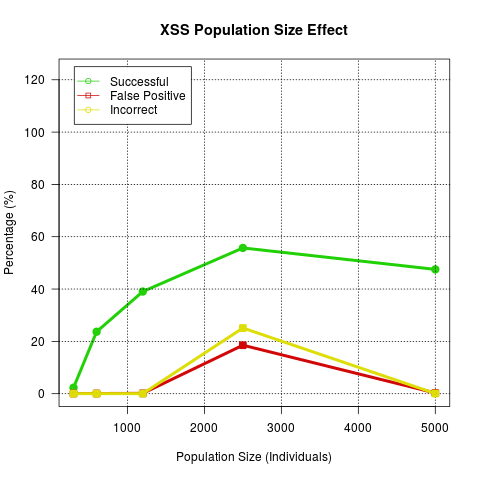
\includegraphics[height=225px]{./assets/appendix/fullresults/ga/pop/Results_XSS.png}
	\caption{Effects of Population Size on Detecting XSS}
	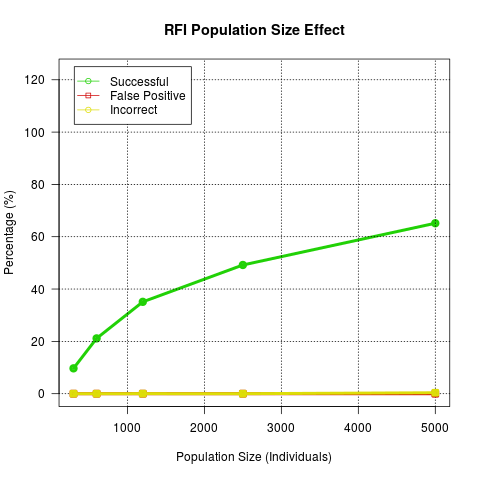
\includegraphics[height=225px]{./assets/appendix/fullresults/ga/pop/Results_RFI.png}
	\caption{Effects of Population Size on Detecting RFI}
\end{figure}

\newpage
\subsection{Generations} \label{app:resGeneration}

\begin{figure}[hp]
	\centering
	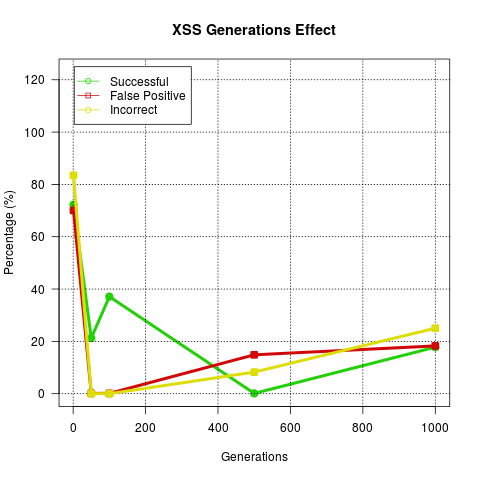
\includegraphics[height=225px]{./assets/appendix/fullresults/ga/generations/Results_XSS.png}
	\caption{Effects of Number of Generations on Detecting XSS}
	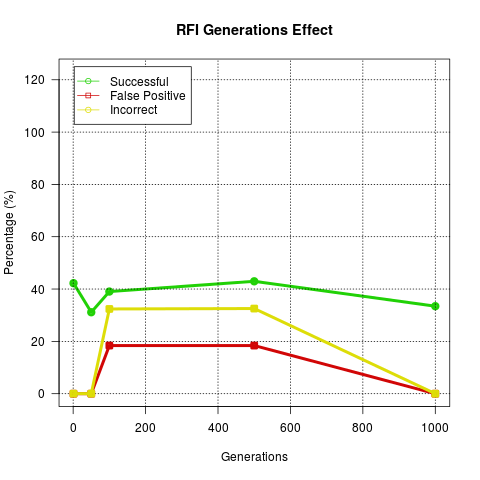
\includegraphics[height=225px]{./assets/appendix/fullresults/ga/generations/Results_RFI.png}
	\caption{Effects of Number of Generations on Detecting RFI}
\end{figure}

\newpage
\subsection{Mutation Rate} \label{app:resMutation}

\begin{figure}[hp]
	\centering
	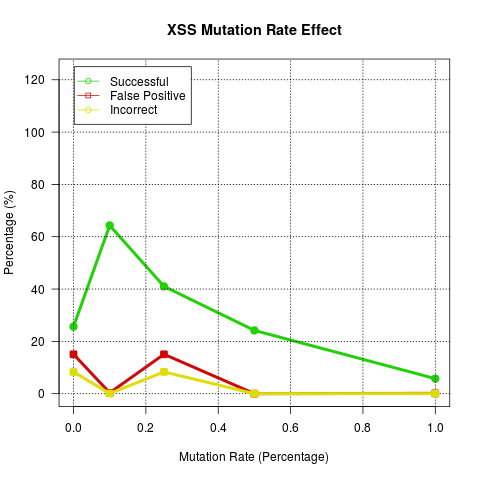
\includegraphics[height=225px]{./assets/appendix/fullresults/ga/mutation/Results_XSS.png}
	\caption{Effects of Mutation Rate on Detecting XSS}
	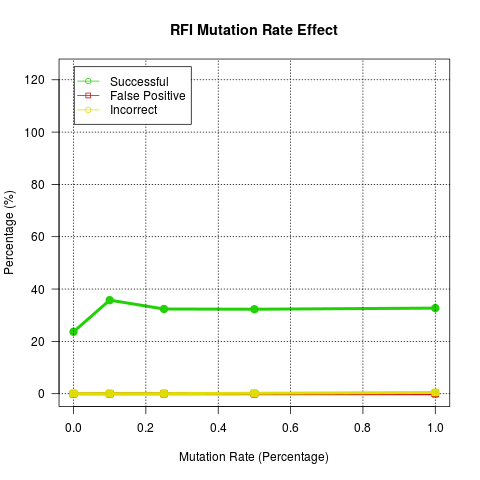
\includegraphics[height=225px]{./assets/appendix/fullresults/ga/mutation/Results_RFI.png}
	\caption{Effects of Mutation Rate on Detecting RFI}
\end{figure}

\newpage
\subsection{Elitist Pool} \label{app:resElitist}

\begin{figure}[hp]
	\centering
	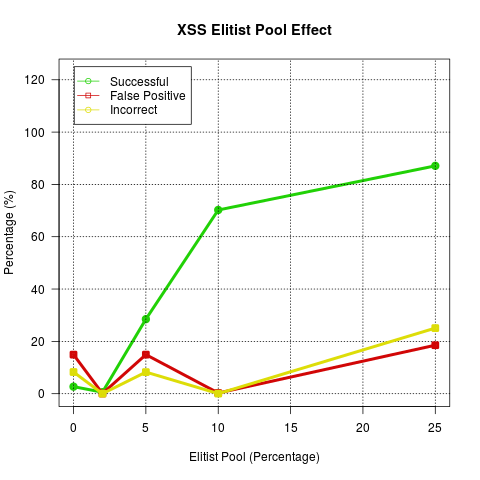
\includegraphics[height=225px]{./assets/appendix/fullresults/ga/elitist/Results_XSS.png}
	\caption{Effects of Elitist Pool on Detecting XSS}
	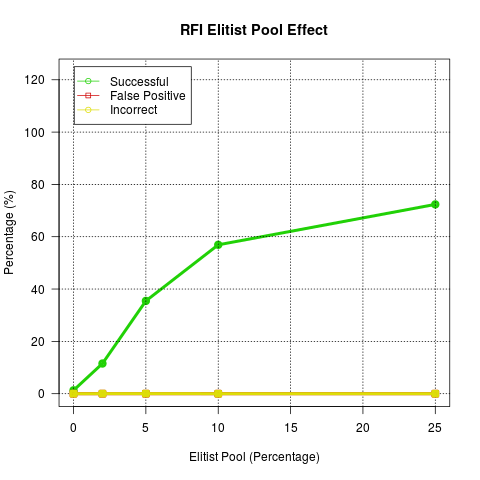
\includegraphics[height=225px]{./assets/appendix/fullresults/ga/elitist/Results_RFI.png}
	\caption{Effects of Elitist Pool on Detecting RFI}
\end{figure}

\newpage
\subsection{Combining Multiple Signature Sets} \label{app:resIteration}

\begin{figure}[hp]
	\centering
	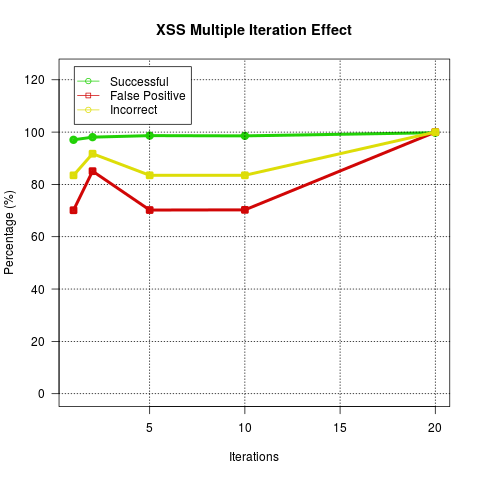
\includegraphics[height=225px]{./assets/appendix/fullresults/ga/iterations/Results_XSS.png}
	\caption{Effects of Multiple Iterations on Detecting XSS}
	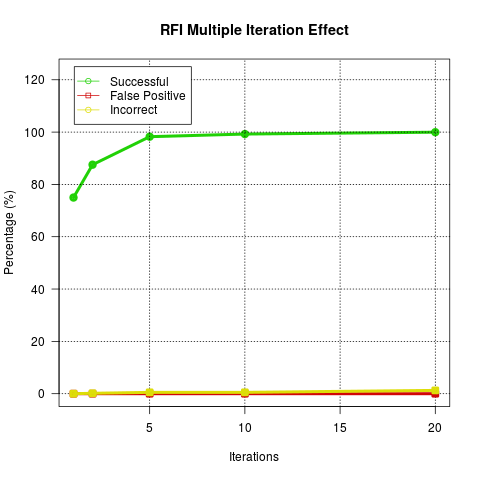
\includegraphics[height=225px]{./assets/appendix/fullresults/ga/iterations/Results_RFI.png}
	\caption{Effects of Multiple Iterations on Detecting RFI}
\end{figure}

\newpage
\subsection{Bitstring Segment Length Effects} \label{app:resSegment}

\begin{figure}[hp]
	\centering
	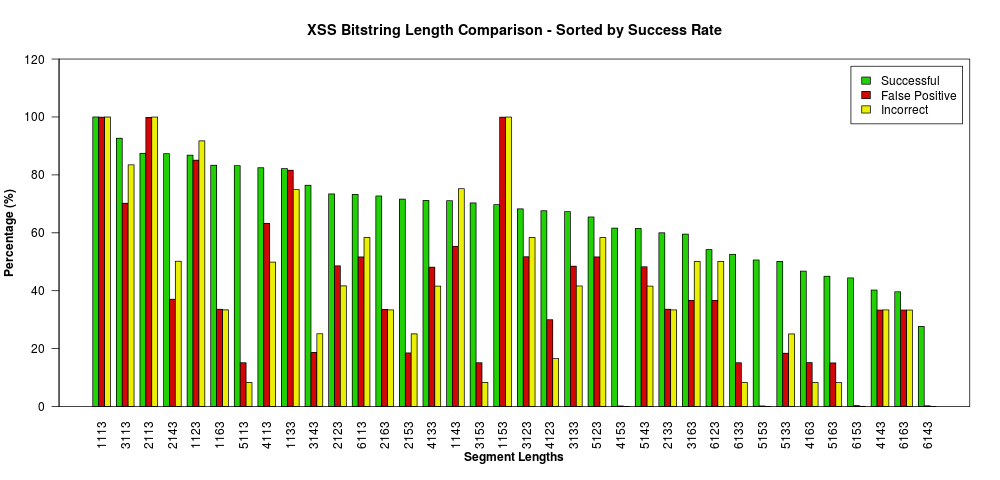
\includegraphics[height=225px]{./assets/appendix/fullresults/ga/bitlength/Results_SuccessRate_XSS.png}
	\caption{Effects of Segment Lengths on Detecting XSS}
	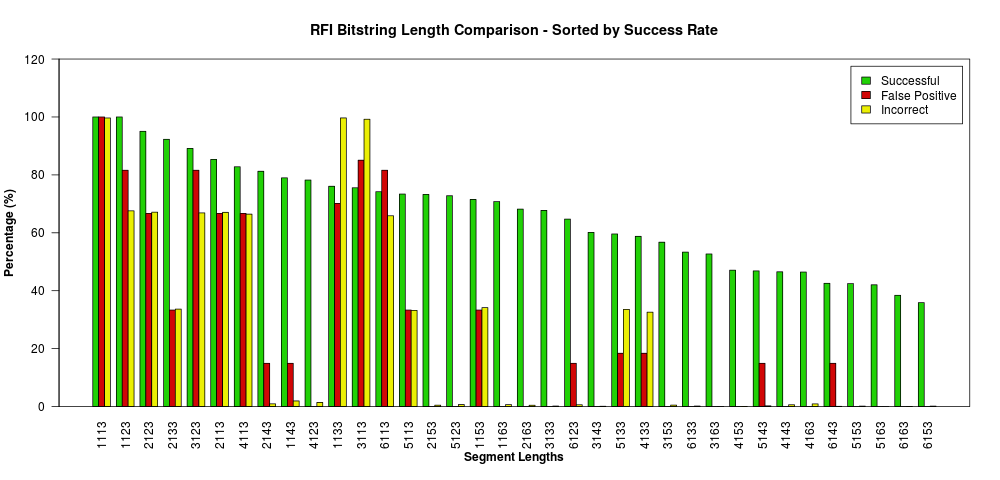
\includegraphics[height=225px]{./assets/appendix/fullresults/ga/bitlength/Results_SuccessRate_RFI.png}
	\caption{Effects of Segment Lengths on Detecting RFI}
\end{figure}

\newpage
\subsection{Compared With Random Permutations with Fitness} \label{app:resRand}

\begin{figure}[hp]
	\centering
	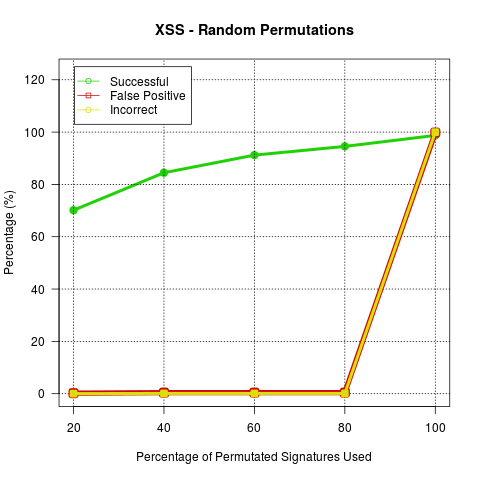
\includegraphics[height=225px]{./assets/appendix/fullresults/rand/Results_XSS.png}
	\caption{Random Permutations to Detecting XSS}
	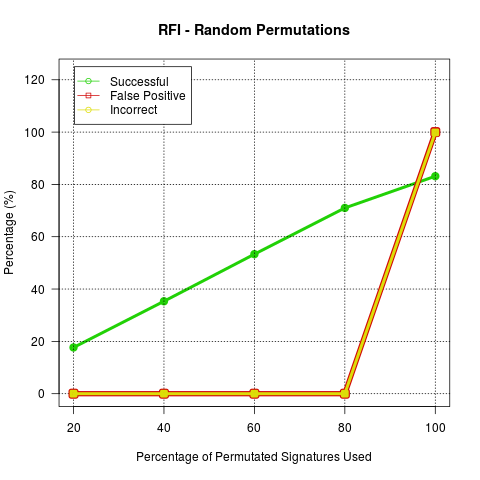
\includegraphics[height=225px]{./assets/appendix/fullresults/rand/Results_RFI.png}
	\caption{Random Permutations to Detecting RFI}
\end{figure}

\chapter{Full Support Vector Machine Testing Results} \label{app:svmFullResults}

\section{Full Text-Based Results}
\subsection{Comparison with Genetic Algorithm}

\begin{longtable}{|p{1.5in}|p{1in}|p{1in}|p{1in}|}
	\hline
	\textbf{Training Info \& Kernel Info} & \textbf{Successful Detection Rate (\%)} & \textbf{False Positive Rate (\%)} & \textbf{Incorrect Detection Rate (\%)}  \\
	\hhline{|=|=|=|=|}
	1000\_334L 	& 90.26 & 11.20 & 5.00 \\ \hline
	1000\_334P 	& 47.46 &  1.80 & 0.66 \\ \hline
	1000\_334R 	& 90.06 &  5.00 & 4.53 \\ \hline
	150\_50L 	& 90.26 & 11.20 & 5.50 \\ \hline
	150\_50P 	& 47.60 &  2.00 & 0.86 \\ \hline
	150\_50R 	& 90.00 &  5.00 & 4.66 \\ \hline
	300\_100L 	& 90.26 & 11.20 & 5.00 \\ \hline
	300\_100P 	& 54.53 &  2.20 & 2.06 \\ \hline
	300\_100R 	& 90.00 &  5.00 & 4.66 \\ \hline
	420\_140L 	& 90.26 & 11.20 & 5.00 \\ \hline
	420\_140P 	& 79.13 &  2.60 & 2.53 \\ \hline
	420\_140R 	& 90.00 &  5.00 & 4.66 \\ \hline
	562\_189L 	& 90.26 & 11.20 & 5.00 \\ \hline
	562\_189P 	& 54.80 &  2.20 & 2.06 \\ \hline
	562\_189R 	& 90.00 &  5.00 & 4.66 \\ \hline
	750\_250L 	& 90.26 & 11.20 & 5.00 \\ \hline
	750\_250P 	& 47.13 &  1.80 & 0.66 \\ \hline
	750\_250R 	& 90.00 &  5.00 & 4.66 \\ \hline
	75\_25L 		& 90.26 & 11.20 & 5.00 \\ \hline
	75\_25P 		& 79.00 &  8.80 & 2.33 \\ \hline
	75\_25R 		& 90.33 & 11.20 & 6.36 \\ \hline
	\caption{Text based effects of genetic algorithm and SVM comparison on SQLi detection}
\end{longtable}

\begin{longtable}{|p{1.5in}|p{1in}|p{1in}|p{1in}|}
	\hline
	\textbf{Training Info \& Kernel Info} & \textbf{Successful Detection Rate (\%)} & \textbf{False Positive Rate (\%)} & \textbf{Incorrect Detection Rate (\%)}  \\
	\hhline{|=|=|=|=|}
	 1000\_334L & 90.86 & 0.20 & 0.03 \\ \hline
	 1000\_334P & 90.86 & 0.20 & 0.03 \\ \hline
	 1000\_334R & 90.86 & 0.20 & 0.03 \\ \hline
	   150\_50L & 90.86 & 0.20 & 0.03 \\ \hline
	   150\_50P & 90.86 & 0.20 & 0.03 \\ \hline
	   150\_50R & 90.86 & 0.20 & 0.03 \\ \hline
	  300\_100L & 90.86 & 0.20 & 0.03 \\ \hline
	  300\_100P & 90.86 & 0.20 & 0.03 \\ \hline
	  300\_100R & 90.86 & 0.20 & 0.03 \\ \hline
	  420\_140L & 90.86 & 0.20 & 0.03 \\ \hline
	  420\_140P & 90.86 & 0.20 & 0.03 \\ \hline
	  420\_140R & 90.86 & 0.20 & 0.03 \\ \hline
	  562\_189L & 90.86 & 0.20 & 0.03 \\ \hline
	  562\_189P & 90.86 & 0.20 & 0.03 \\ \hline
	  562\_189R & 90.86 & 0.20 & 0.03 \\ \hline
	  750\_250L & 90.86 & 0.20 & 0.03 \\ \hline
	  750\_250P & 90.86 & 0.20 & 0.03 \\ \hline
	  750\_250R & 90.86 & 0.20 & 0.03 \\ \hline
	    75\_25L & 90.86 & 0.20 & 0.03 \\ \hline
	    75\_25P & 90.86 & 0.20 & 0.03 \\ \hline
	    75\_25R & 90.86 & 0.20 & 0.03 \\ \hline
	\caption{Text based effects of genetic algorithm and SVM comparison on XSS detection}
\end{longtable}

\begin{longtable}{|p{1.5in}|p{1in}|p{1in}|p{1in}|}
	\hline
	\textbf{Training Info \& Kernel Info} & \textbf{Successful Detection Rate (\%)} & \textbf{False Positive Rate (\%)} & \textbf{Incorrect Detection Rate (\%)}  \\
	\hhline{|=|=|=|=|}
	1000\_334L &  99.20 & 0.00 & 0.16 \\ \hline
	1000\_334P &  99.20 & 0.00 & 0.00 \\ \hline
	1000\_334R & 100.00 & 0.00 & 0.03 \\ \hline
	150\_50L & 100.00 & 0.00 & 0.16 \\ \hline
	150\_50P &  99.20 & 0.00 & 0.06 \\ \hline
	150\_50R & 100.00 & 0.00 & 0.06 \\ \hline
	300\_100L &  99.20 & 0.00 & 0.16 \\ \hline
	300\_100P &  99.20 & 0.00 & 0.00 \\ \hline
	300\_100R & 100.00 & 0.00 & 0.00 \\ \hline
	420\_140L &  99.20 & 0.00 & 0.16 \\ \hline
	420\_140P &  99.20 & 0.00 & 0.00 \\ \hline
	420\_140R & 100.00 & 0.00 & 0.06 \\ \hline
	562\_189L & 100.00 & 0.00 & 0.53 \\ \hline
	562\_189P &  99.20 & 0.00 & 0.00 \\ \hline
	562\_189R & 100.00 & 0.00 & 0.06 \\ \hline
	750\_250L & 100.00 & 0.00 & 0.56 \\ \hline
	750\_250P &  99.20 & 0.00 & 0.00 \\ \hline
	750\_250R & 100.00 & 0.00 & 0.03 \\ \hline
	75\_25L &  99.20 & 0.00 & 0.16 \\ \hline
	75\_25P &  97.66 & 0.00 & 0.03 \\ \hline
	75\_25R &  99.20 & 0.00 & 0.26 \\ \hline
	\caption{Text based effects of genetic algorithm and SVM comparison on RFI detection}
\end{longtable}

\newpage
\subsection{Increasing Non-Threats}

\begin{longtable}{|p{1.5in}|p{1in}|p{1in}|p{1in}|}
	\hline
	\textbf{Training Info \& Kernel Info} & \textbf{Successful Detection Rate (\%)} & \textbf{False Positive Rate (\%)} & \textbf{Incorrect Detection Rate (\%)}  \\
	\hhline{|=|=|=|=|}
 	100L & 90.26 & 11.20 &  5.00 \\ \hline
 	100P & 54.53 &  2.20 &  2.06 \\ \hline
 	100R & 90.00 &  5.00 &  4.66 \\ \hline
 	200L & 90.33 &  7.20 &  6.36 \\ \hline
 	200P & 47.33 &  2.00 &  0.86 \\ \hline
 	200R & 90.33 & 11.20 &  6.36 \\ \hline
 	350L & 90.33 &  5.20 &  6.36 \\ \hline
 	350P & 47.60 &  2.20 &  0.86 \\ \hline
 	350R & 90.33 &  7.20 &  6.26 \\ \hline
 	500L & 99.13 &  6.60 & 15.90 \\ \hline
 	500P & 47.60 &  2.20 &  0.86 \\ \hline
 	500R & 90.13 &  5.20 &  5.60 \\ \hline
  	50L & 90.26 & 11.20 &  5.00 \\ \hline
  	50P & 54.53 &  2.20 &  2.06 \\ \hline
  	50R & 90.00 &  5.00 &  4.70 \\ \hline
 	750L & 79.26 &  3.00 &  3.90 \\ \hline
 	750P & 47.60 &  2.20 &  0.86 \\ \hline
 	750R & 90.00 &  5.00 &  4.66 \\ \hline
 	\caption{Text based effects of increasing non-threats in training data on SQLi detection}
\end{longtable}

\begin{longtable}{|p{1.5in}|p{1in}|p{1in}|p{1in}|}
	\hline
	\textbf{Training Info \& Kernel Info} & \textbf{Successful Detection Rate (\%)} & \textbf{False Positive Rate (\%)} & \textbf{Incorrect Detection Rate (\%)}  \\
	\hhline{|=|=|=|=|}
 	100L & 90.86 & 0.20 & 0.03 \\ \hline
 	100P & 90.86 & 0.20 & 0.03 \\ \hline
 	100R & 90.86 & 0.20 & 0.03 \\ \hline
 	200L & 90.86 & 0.20 & 0.03 \\ \hline
 	200P & 90.86 & 0.20 & 0.03 \\ \hline
 	200R & 90.86 & 0.20 & 0.03 \\ \hline
 	350L & 90.86 & 0.20 & 0.03 \\ \hline
 	350P & 90.86 & 0.20 & 0.03 \\ \hline
 	350R & 90.86 & 0.20 & 0.03 \\ \hline
 	500L & 90.86 & 0.20 & 0.03 \\ \hline
 	500P & 90.86 & 0.20 & 0.03 \\ \hline
 	500R & 90.86 & 0.20 & 0.03 \\ \hline
  	50L & 90.86 & 0.20 & 0.03 \\ \hline
  	50P & 90.86 & 0.20 & 0.03 \\ \hline
  	50R & 90.86 & 0.20 & 0.03 \\ \hline
 	750L & 90.86 & 0.20 & 0.03 \\ \hline
 	750P & 90.86 & 0.20 & 0.03 \\ \hline
 	750R & 90.86 & 0.20 & 0.03 \\ \hline
 	\caption{Text based effects of increasing non-threats in training data on XSS detection}
\end{longtable}
	
\begin{longtable}{|p{1.5in}|p{1in}|p{1in}|p{1in}|}
	\hline
	\textbf{Training Info \& Kernel Info} & \textbf{Successful Detection Rate (\%)} & \textbf{False Positive Rate (\%)} & \textbf{Incorrect Detection Rate (\%)}  \\
	\hhline{|=|=|=|=|}
	100L &  99.20 &  0.00 &  0.16 \\ \hline
	100P &  99.20 &  0.00 &  0.00 \\ \hline
	100R & 100.00 &  0.00 &  0.00 \\ \hline
	200L &  99.20 &  0.00 &  0.16 \\ \hline
	200P &  97.66 &  0.00 &  0.00 \\ \hline
	200R &  99.20 &  0.00 &  0.26 \\ \hline
	350L &  99.20 &  0.00 &  0.16 \\ \hline
	350P &  99.20 &  0.00 &  0.00 \\ \hline
	350R &  99.20 &  0.00 &  0.26 \\ \hline
	500L &  99.20 &  0.00 &  0.16 \\ \hline
	500P &  99.20 &  0.00 &  0.00 \\ \hline
	500R &  99.20 &  0.00 &  0.16 \\ \hline
 	50L &  99.20 &  0.00 &  0.16 \\ \hline
 	50P &  99.20 &  0.00 &  0.00 \\ \hline
 	50R & 100.00 &  0.00 &  0.00 \\ \hline
	750L &  99.20 &  0.00 &  0.16 \\ \hline
	750P &  99.20 &  0.00 &  0.00 \\ \hline
	750R &  99.20 &  0.00 &  0.10 \\ \hline
	\caption{Text based effects of increasing non-threats in training data on RFI detection}
\end{longtable}

\newpage
\subsection{Increasing Incorrect-Threats}

\begin{longtable}{|p{1.5in}|p{1in}|p{1in}|p{1in}|}
	\hline
	\textbf{Training Info \& Kernel Info} & \textbf{Successful Detection Rate (\%)} & \textbf{False Positive Rate (\%)} & \textbf{Incorrect Detection Rate (\%)}  \\
	\hhline{|=|=|=|=|}
 	100L & 99.13 & 6.60 & 15.90 \\ \hline
 	100P & 90.26 & 4.60 &  6.36 \\ \hline
 	100R & 99.13 & 7.00 & 15.90 \\ \hline
 	200L & 99.13 & 6.60 & 15.90 \\ \hline
 	200P & 54.86 & 2.20 &  2.06 \\ \hline
 	200R & 90.33 & 7.20 &  6.30 \\ \hline
 	275L & 99.13 & 7.00 & 15.90 \\ \hline
 	275P & 47.60 & 2.20 &  0.86 \\ \hline
 	275R & 90.33 & 7.20 &  6.26 \\ \hline
 	350L & 79.26 & 5.20 &  3.90 \\ \hline
 	350P & 47.33 & 2.00 &  0.86 \\ \hline
 	350R & 90.33 & 7.20 &  6.26 \\ \hline
  	50L & 99.13 & 6.60 & 15.90 \\ \hline
  	50P & 99.13 & 7.00 & 15.90 \\ \hline
  	50R & 99.13 & 7.00 & 15.90 \\ \hline
 	600L & 79.20 & 5.00 &  2.53 \\ \hline
 	600P & 40.13 & 1.40 &  0.66 \\ \hline
 	600R & 90.00 & 7.20 &  4.70 \\ \hline
 	750L & 54.86 & 4.40 &  2.06 \\ \hline
 	750P & 31.40 & 1.80 &  0.23 \\ \hline
 	750R & 90.00 & 5.00 &  4.66 \\ \hline
 	\caption{Text based effects of increasing incorrect-threats in training data on SQLi detection}
\end{longtable}
	
\begin{longtable}{|p{1.5in}|p{1in}|p{1in}|p{1in}|}
	\hline
	\textbf{Training Info \& Kernel Info} & \textbf{Successful Detection Rate (\%)} & \textbf{False Positive Rate (\%)} & \textbf{Incorrect Detection Rate (\%)}  \\
	\hhline{|=|=|=|=|}
 	100L & 90.86 & 0.20 & 0.03 \\ \hline
 	100P & 90.86 & 0.20 & 0.03 \\ \hline
 	100R & 90.86 & 0.20 & 0.03 \\ \hline
 	200L & 90.86 & 0.20 & 0.03 \\ \hline
 	200P & 90.86 & 0.20 & 0.03 \\ \hline
 	200R & 90.86 & 0.20 & 0.03 \\ \hline
 	275L & 90.86 & 0.20 & 0.03 \\ \hline
 	275P & 56.93 & 0.20 & 0.03 \\ \hline
 	275R & 90.86 & 0.20 & 0.03 \\ \hline
 	350L & 90.86 & 0.20 & 0.03 \\ \hline
 	350P & 90.86 & 0.20 & 0.03 \\ \hline
 	350R & 90.86 & 0.20 & 0.03 \\ \hline
  	50L & 90.86 & 0.20 & 0.03 \\ \hline
  	50P & 56.93 & 0.20 & 0.03 \\ \hline
  	50R & 90.86 & 0.20 & 0.03 \\ \hline
 	600L & 90.86 & 0.20 & 0.03 \\ \hline
 	600P & 90.86 & 0.20 & 0.03 \\ \hline
 	600R & 90.86 & 0.20 & 0.03 \\ \hline
 	750L & 90.86 & 0.20 & 0.03 \\ \hline
 	750P & 90.86 & 0.20 & 0.03 \\ \hline
 	750R & 90.86 & 0.20 & 0.03 \\ \hline
 	\caption{Text based effects of increasing incorrect-threats in training data on XSS detection}
\end{longtable}

\begin{longtable}{|p{1.5in}|p{1in}|p{1in}|p{1in}|}
	\hline
	\textbf{Training Info \& Kernel Info} & \textbf{Successful Detection Rate (\%)} & \textbf{False Positive Rate (\%)} & \textbf{Incorrect Detection Rate (\%)}  \\
	\hhline{|=|=|=|=|}
	100L & 100.00 &  0.00 & 0.73 \\ \hline
	100P &  99.20 &  0.00 & 0.06 \\ \hline
	100R & 100.00 &  0.00 & 0.26 \\ \hline
	200L &  99.20 &  0.00 & 0.16 \\ \hline
	200P &  99.20 &  0.00 & 0.06 \\ \hline
	200R & 100.00 &  0.00 & 0.56 \\ \hline
	275L &  99.20 &  0.00 & 0.16 \\ \hline
	275P &  97.66 &  0.00 & 0.03 \\ \hline
	275R &  99.20 &  0.00 & 0.16 \\ \hline
	350L &  99.20 &  0.00 & 0.16 \\ \hline
	350P &  99.20 &  0.00 & 0.00 \\ \hline
	350R &  99.20 &  0.00 & 0.16 \\ \hline
	 50L & 100.00 &  0.00 & 0.10 \\ \hline
	 50P &  99.20 &  0.00 & 0.06 \\ \hline
	 50R & 100.00 &  0.00 & 0.10 \\ \hline
	600L &  99.20 &  0.00 & 0.10 \\ \hline
	600P &  99.20 &  0.00 & 0.00 \\ \hline
	600R &  99.20 &  0.00 & 0.16 \\ \hline
	750L &  99.20 &  0.00 & 0.10 \\ \hline
	750P &  99.20 &  0.00 & 0.00 \\ \hline
	750R &  99.20 &  0.00 & 0.16 \\ \hline
	\caption{Text based effects of increasing incorrect-threats in training data on RFI detection}
\end{longtable}

\newpage
\section{Remaining Graphical Results}
\subsection{Comparison with Genetic Algorithm} \label{app:resComparison}

\begin{figure}[hp]
	\centering
	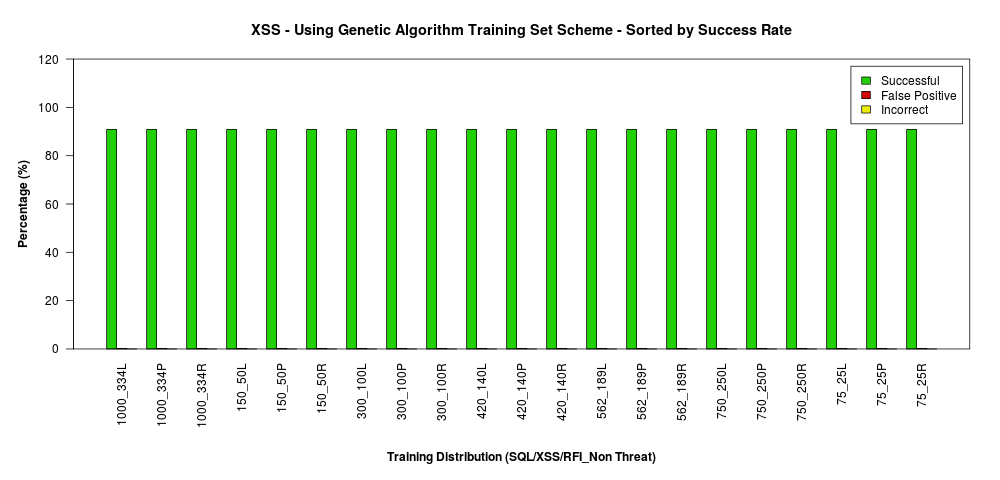
\includegraphics[height=225px]{./assets/appendix/fullresults/svm/comparison/Results_XSS.png}
	\caption{Genetic Algorithm and SVM comparison for Detecting XSS}
	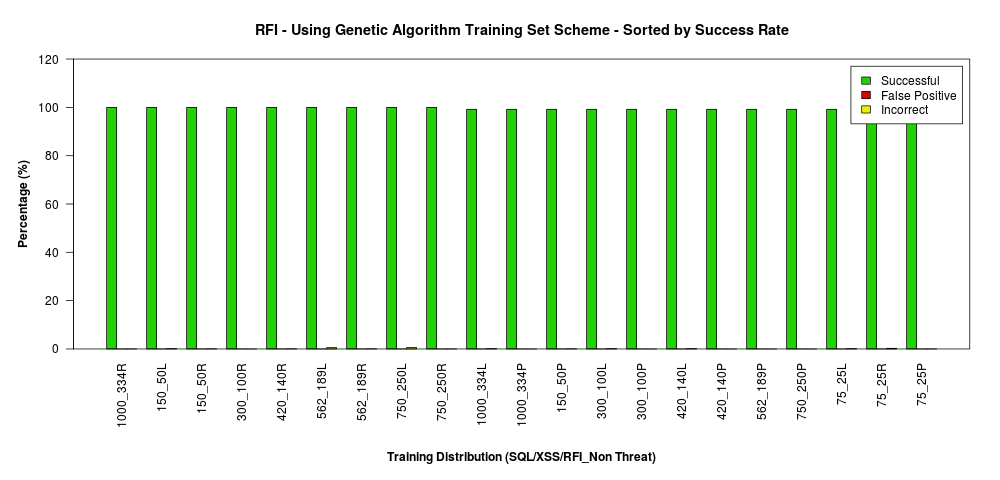
\includegraphics[height=225px]{./assets/appendix/fullresults/svm/comparison/Results_RFI.png}
	\caption{Genetic Algorithm and SVM comparison for Detecting RFI}
\end{figure}

\newpage
\subsection{Increasing Non-Threats}  \label{app:resNonThreat}

\begin{figure}[hp]
	\centering
	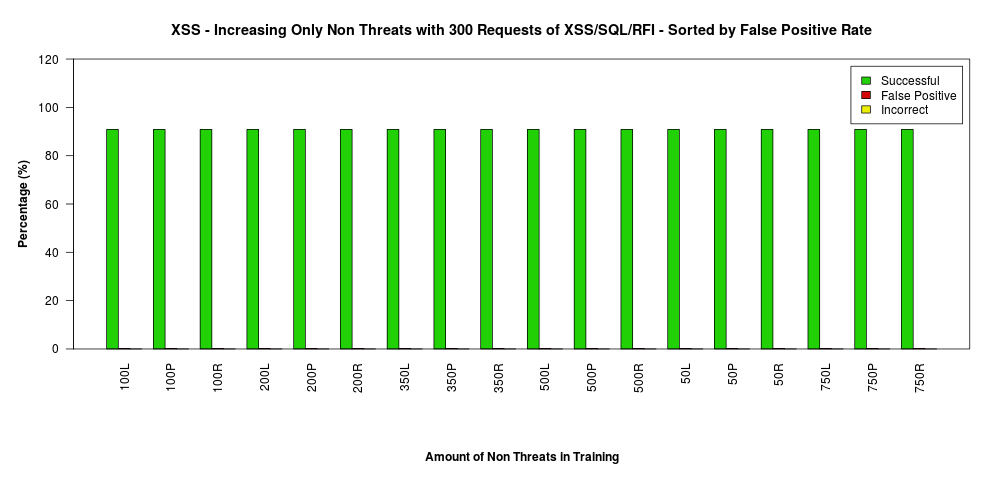
\includegraphics[height=225px]{./assets/appendix/fullresults/svm/nonthreat/Results_XSS.png}
	\caption{Effects of Increasing Non-Threat training data in Detecting XSS}
	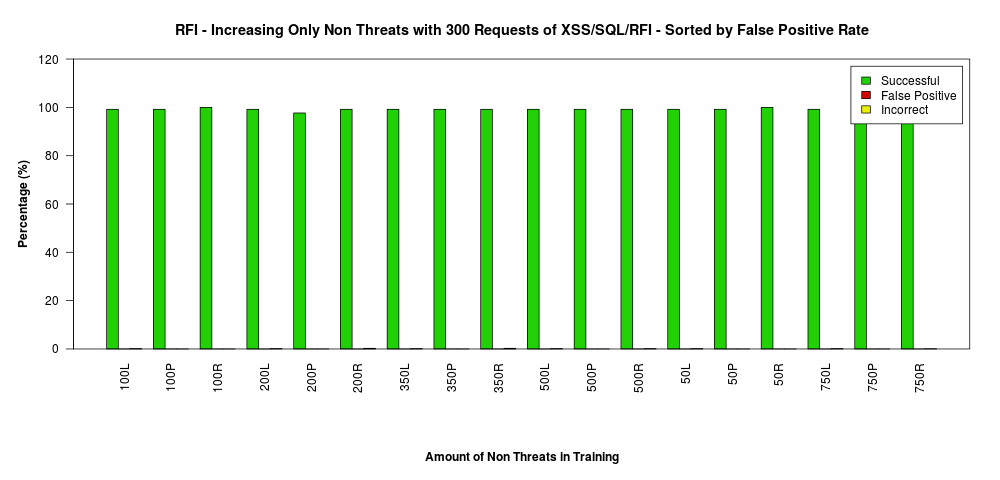
\includegraphics[height=225px]{./assets/appendix/fullresults/svm/nonthreat/Results_RFI.png}
	\caption{Effects of Increasing Non-Threat training data in Detecting RFI}
\end{figure}

\newpage
\subsection{Increasing Incorrect-Threats} \label{app:resIncorrect}

\begin{figure}[hp]
	\centering
	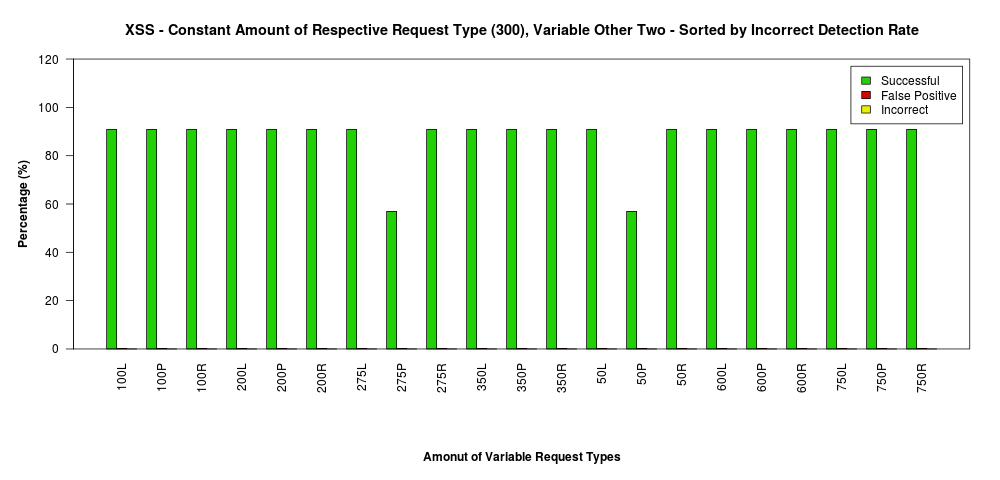
\includegraphics[height=225px]{./assets/appendix/fullresults/svm/incorrect/Results_XSS.png}
	\caption{Effects of Increasing incorrect attack type training data in Detecting XSS}
	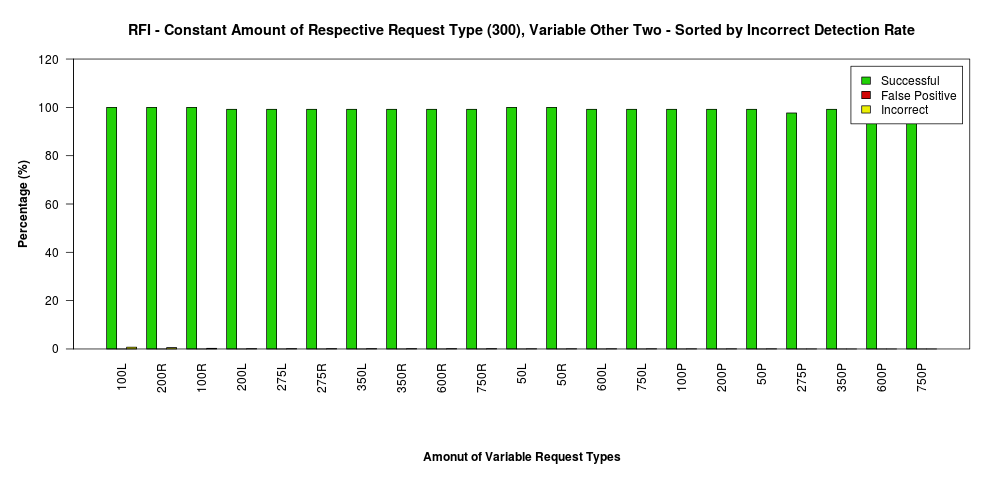
\includegraphics[height=225px]{./assets/appendix/fullresults/svm/incorrect/Results_RFI.png}
	\caption{Effects of Increasing incorrect attack type training data in Detecting RFI}
\end{figure}

\end{appendices}
